\documentclass[12pt,twocolumn]{IEEEtran}
\usepackage{ifpdf}
\usepackage{graphicx}
\usepackage{cite}
\usepackage{listings}
\usepackage{color}
\usepackage{subcaption}

\definecolor{mygreen}{rgb}{0,0.6,0}
\definecolor{mygray}{rgb}{0.5,0.5,0.5}
\definecolor{mymauve}{rgb}{0.58,0,0.82}

\lstset{ 
	backgroundcolor=\color{white},   % choose the background color; you must add \usepackage{color} or \usepackage{xcolor}; should come as last argument
	basicstyle=\footnotesize,        % the size of the fonts that are used for the code
	breakatwhitespace=true,          % sets if automatic breaks should only happen at whitespace
	breaklines=true,                 % sets automatic line breaking
	captionpos=b,                    % sets the caption-position to bottom
	commentstyle=\color{mygreen},    % comment style
	deletekeywords={...},            % if you want to delete keywords from the given language
	escapeinside={\%*}{*)},          % if you want to add LaTeX within your code
	extendedchars=true,              % lets you use non-ASCII characters; for 8-bits encodings only, does not work with UTF-8
	firstnumber=1,                   % start line enumeration with line 1
	frame=single,                    % adds a frame around the code
	keepspaces=true,                 % keeps spaces in text, useful for keeping indentation of code (possibly needs columns=flexible)
	keywordstyle=\color{blue},       % keyword style
	language=Java,                   % the language of the code
	morekeywords={*,...},            % if you want to add more keywords to the set
	numbers=left,                    % where to put the line-numbers; possible values are (none, left, right)
	numbersep=5pt,                   % how far the line-numbers are from the code
	numberstyle=\tiny\color{mygray}, % the style that is used for the line-numbers
	rulecolor=\color{black},         % if not set, the frame-color may be changed on line-breaks within not-black text (e.g. comments (green here))
	showspaces=false,                % show spaces everywhere adding particular underscores; it overrides 'showstringspaces'
	showstringspaces=false,          % underline spaces within strings only
	showtabs=false,                  % show tabs within strings adding particular underscores
	stepnumber=5,                    % the step between two line-numbers. If it's 1, each line will be numbered
	stringstyle=\color{mymauve},     % string literal style
	tabsize=1,	                   % sets default tabsize to 2 spaces
	title=\lstname                   % show the filename of files included with \lstinputlisting; also try caption instead of title
}

\ifpdf
\pdfinfo{
	/Title (Analysis of Dependency Injection Frameworks in Java and their Features)
	/Author (Nicholas Kastanos (1393410))
	/CreationDate (D:201902211949)
	/ModDate (D:201903281109)
	/Subject (Software 3 Report)
	/Keywords (dependency injection, java, framework)
}
\fi

\begin{document}
	\onecolumn
	\title{Analysis of Dependency Injection Frameworks in Java and their Features}
	
	\author{\IEEEauthorblockN{Nicholas Kastanos (1393410)}\\
		\IEEEauthorblockA{School of Electrical \& Information Engineering, University of the Witwatersrand, Private Bag 3, 2050, Johannesburg, South Africa\\ELEN4010 Software Development III\\1 April 2019}}
	
	\maketitle
	
	\begin{abstract}
		Dependency Injection Frameworks are used to assist software developers in creating programs which follow the Dependency Inversion Principle and Inversion of Control Principle. Three Java-based frameworks are analysed, and their features are classified into two categories: Essential, and Supplementary features. A sample program is created using Guice to demonstrate the capabilities of the framework, and the advantages and disadvantages of using a Dependency Injection framework are discussed.
	\end{abstract}

\thispagestyle{empty}
\setcounter{page}{0}
\twocolumn
\clearpage

\section{Introduction}

Tight coupling of dependent code can create issues when code implementation is altered, and is hard to test and maintain. One method of reducing the coupling of dependencies is by making use of a framework to implement Dependency Injection. Different Dependency Injection frameworks provide different features, and there is no consensus on which features are considered essential or supplementary. Dependency Injection can be implemented in any language, however the Dependency Injection frameworks Spring Framework, Guice, and Dagger 2 are all implemented for Java code. These frameworks are analysed and their features are categorised, and their effectiveness are analysed.

Sections~\ref{sec:di}~and~\ref{sec:dif} describe Dependency Injection and the frameworks which implement them. Section~\ref{sec:features} highlights the key features of these frameworks, and classifies them. An example of a program implemented using Guice is shown in Section~\ref{sec:guice}, and Dependency Injection frameworks are analysed in Section~\ref{sec:analysis}.

\section{Dependency Injection}\label{sec:di}

The origins of Dependency Injection are rooted in the concepts of the \textit{Dependency Inversion Principle} (DIP) which was first discussed by Martin in 1996 \cite{martin1996}, and the \textit{Inversion of Control} (IoC) principle, by Foote \cite{foote1988}. 

%"High-level modules should not depend upon low-level modules. Both should depend upon abstractions" R. C. Martin. The Dependency Inversion Principle. C++ Report, 8(6):61–66, June 1996.

% IoC --------------- R. E. Johnson and B. Foote. Designing reusable classes. Journal of Object-Oriented Programming, 1(2):22–35, 1988.

These principles state that classes should not depend on other concrete classes, but should only depend on abstract interfaces. This allows the programmer to avoid what Martin describes as a ``Bad Design'', and avoids rigidity, frailty, and immobility in the code.

By having classes depend on abstract interfaces, the implementation of the dependencies can be easily altered without needing the change the code of the class. This makes the code more flexible and less fragile, leading the easier future developments or changes. 

Dependency Injection (DI) provides the solution to this problem by linking the required implementation to the interface without the dependant class having to have knowledge of which implementation is being used \cite{tonymarston2016,hongyulyangewantemperohaydenmelton2008}. 

% MAYBE TALK ABOUT ORDERS OF LAYERS AND DEPENDENCIES AND HOW DI MAKES THIS BETTER.
It is possible to implement DI using the standard libraries for many languages, however this requires well structured and planned code, and can become complicated and prone to errors in large programs. In order to simplify the inclusion of DI in code, many DI Frameworks have been developed.

\section{DI Frameworks}\label{sec:dif}

% Talk about frameworks in general, and then DI frameworks. How do they help implement DI and IoC effectively.
DI frameworks are structured to encourage good use of the underlying principles \cite{rodjohnson2005,dennisdoomen2018}, and are designed to make the use of DI easy and simple. DI Frameworks in Java are usually implemented in two structures: XML configuration files, or Injector Java objects. Some of the more popular DI frameworks are discussed below.
% Many Dependency Injection Frameworks are designed to make the implementation of IoC and DIP principles into a unified and simple

Spring Framework is a comprehensive framework which provides more functionality than DI. It also supports features such as data binding, database connections, and web framework support. The DI framework section of Spring makes use of both Plain Old Java Objects (POJO) and XML files to configure the bindings and injections \cite{spring2019}.
% https://docs.spring.io/spring-framework/docs/current/spring-framework-reference/core.html#beans-factory-collaborators

Guice is a lightweight DI Framework developed by Google to provide fast and simple DI using POJO principles. Unlike Spring Framework, Guice only provides DI capabilities \cite{guicewiki2014}.

Dagger 2 is a DI-only framework which is fully static and is implemented at compile time. This fully implements the program's stack at compile time which allows for easier debugging and faster run-times. Additionally it as able to run on Android systems, which increases the reach of the framework \cite{dagger2019}.
% https://google.github.io/dagger/

\section{Features of DI Frameworks} \label{sec:features}
Many DI frameworks have both similar and different features or types of DI which it can implement. These features can either be classified as Essential Features or Supplementary Features.

Essential Features are central to implementing the DIP and IoC principles, and are generally included in every DI Framework. Supplementary Features, however, provide additional utility or Quality of Life improvements to assist in implementing more complicated DI structures. 

% https://www.vogella.com/tutorials/SpringDependencyInjection/article.html

\subsubsection{Constructor Injection} % Guice, Spring, Dagger

Constructor Injection occurs when the object is injected into the constructor as an argument. This allows an object to be provided with the required dependency on construction without violating the DIP. Spring Framework, Guice and Dagger 2 all offer this form of injection \cite{guicewiki2014,spring2019,dagger2019}. 

\subsubsection{Method Injection} % Guice, Spring, Dagger 

Similarly to Constructor Injection, Method Injection occurs when the dependency is passed into a method as an argument. This form of injection differs from Constructor Injection by creating the dependency when the method is called, as opposed to when the object is constructed. This interaction may result in more distributed computational requirements should the construction be computationally expensive. Spring Framework, Guice and Dagger 2 all offer this form of injection \cite{guicewiki2014,spring2019,dagger2019}. 

\subsubsection{Field Injection} % Guice, Dagger

Field Injection allows a dependency to be injected directly into an object's fields. This generally occurs on instantiation of the object, and allows the constructor of the object to be free of some injections. Guice and Dagger 2 contain this functionality \cite{guicewiki2014,dagger2019}.

\subsubsection{Defaults or Optional Injection} % Spring, Guice, Dagger
Default values allow dependency injection to become optional, where the dependency does not have to be created. If the injection does not occur, the program will be able to use a default value for the required dependency. This feature encourages reuse of code, and reduces fatal program errors, however it may increase the amount of logical errors which are present. All three of the frameworks mentioned above have this feature \cite{guicewiki2014,spring2019,dagger2019}.

\subsubsection{Named Linkings} % Guice, Spring, Dagger
This feature allows links between objects and their dependencies to be referred to by more `human readable' names. This increases the readability of code, and does not afford extra functionality. While this does not provide the frameworks with more capabilities, Spring, Guice, and Dagger 2 all support this feature \cite{guicewiki2014,spring2019,dagger2019}.

\subsubsection{Chained Dependencies} % Spring
Chained dependencies occur when one object's dependency contains objects which itself is dependent on. While this is possible to implement using Guice and Dagger 2, Spring Framework provides active support for is feature \cite{spring2019}.

\subsubsection{Provider Injections} % All
Provider injections can be used when multiple values, or objects, need to be provided as a dependency. This ensures than a different instance of the dependency is provided each time. Spring Framework, Guice and Dagger 2 all offer this form of injection \cite{guicewiki2014,spring2019,dagger2019}. 

\subsection{Essential Features}
According to the guidelines set out at the beginning of Section~\ref{sec:features}, Constructor Injection, Method Injection, and Provider Injection are Essential Features for a DI Framework.

Each of these methods of injection provide a framework for implementing the DIP and IoC Principles. Constructor Injection allows dependencies to be set up at the beginning of the object's lifetime, while Method Injection allows the dependencies to be created in the middle of the lifetime. 

Provider Injections are also essential due to the ability to inject large amounts of data and dependencies. Without it, objects would be limited in the amount of dependencies which can be created. 

\subsection{Supplementary Features}

The remaining features, Field and Optional Injection, Named Linkings and Chained Dependencies, can be classified as Supplementary Features. Field Injection can be implemented using Constructor or Method injection by passing a dependency into the objects as a parameter, and setting it to a private member. Optional Injections removes the need for a default injected object, which reduces the complexity of the code. Chained Dependencies can be complicated to program and test without the support of the framework, however it is possible to implement with good programming practice, but may result in longer development times or lower product quality.

\section{Practical Implementation using Guice}\label{sec:guice}

In order to explore the features and usability of DI Frameworks, a sample Java program has been developed using Google's Guice framework (see Appendix~\ref{app:screenshots}~and~\ref{app:code}). % INSERT GIT REPO HERE
The sample program emulates how different payment modules can be integrated into a payment or credit transaction system. The user is presented with a login screen, where a username and password is accepted. Once the user has logged in, the user is placed into a loop where they can repeatedly make transactions until they logout. 

The type of transaction is implemented using the Guice DI Framework. An administrator account can change the \verb|Transaction| class's implementation between a \verb|SecureTransaction|, \verb|FastTransaction|, and \verb|InsecureTransaction|. This implementation is then injected into the \verb|PaymentService|'s constructor via a Provider class, and is used to complete the transaction using different methods. 

% MAYBE ADD MORE THINGS TO THE PROGRAM

While the implementations of the application are fairly trivial, they highlight the capabilities and features of the framework.

\section{Analysis of DI Frameworks}\label{sec:analysis}

The use of DI Frameworks in code affects it in a multitude of ways, as the decoupling of classes leads in increased maintainability, extensibility, and reusability \cite{hongyulyangewantemperohaydenmelton2008,ekaterinarazinadavidjanzen2007}. 

DI Frameworks assist in decoupling dependent objects from one another, which reduces the sensitivity to changes between different parts of the program. This allows the different parts of the program to be changed easily without needing to change other sections of code, increasing flexibility. A program or library which already has clients making use of its interface will not be required to change their own program should the implementation be changed. A side-effect of using the framework is that the code becomes highly dependent on the DI framework, which does limit possible development of the program. Should the framework not support a feature which is essential to an aspect of the program or expansion of the program, the entire application must be reprogrammed to accommodate a new framework.

Since code which is implemented using a DI Framework is highly flexible, the code becomes highly reusable as the implementation can be modified to suit a specific need. The sample application in Section~\ref{sec:guice} which uses DI to change the security level of a transaction can be modified to change the service provider from MasterCard to Visa or a cryptocurrency. 

For many DI Frameworks, the lifetime of the injected objects is controlled by the parent object. This decreases the amount of unnecessary memory usage of the program.

While DI Frameworks provide many benefits, there are drawbacks to using the frameworks. The frameworks each require a specific structure, be that XML files or additional POJO classes. These additional structures take time to learn and implement, increasing the development time of the project. Additionally, the dependencies need to be linked at runtime, which increases the running times of the program. Dagger 2, however, accomplishes all of its linking at compile time, and is significantly more efficient at runtime than other frameworks \cite{androiddeveloperguide}.


\section{Conclusion}

Dependency Injection Frameworks help implement the Dependency Inversion and Inversion of Control Principles, which aim to increase the flexibility and reusability of code. Spring Framework, Guice, and Dagger 2 are examined, their DI features are identified, and classified as either Essential or Supplementary features. 

Constructor Injection, Method Injection, and Provider Injection are deemed as Essential features, while Field and Optional Injection, Named Linkings and Chained Dependencies are classified as Supplementary features.

Guice is then used to demonstrate the functionality of a DI framework, and how it can be used in code. DI Frameworks are found to provide many benefits which include increased maintainability, flexibility, and resuability. However, the running times of the applications are generally slower, and a dependency on the framework is generated.

\bibliographystyle{IEEEtran}
\bibliography{IEEEabrv,references}


\clearpage
\onecolumn
\appendices
\renewcommand\thefigure{\thesection.\arabic{figure}} 
\renewcommand\theequation{\thesection.\arabic{equation}} 
\renewcommand\thetable{\thesection.\arabic{table}}
\renewcommand\thelstlisting{\thesection.\arabic{lstlisting}}
\section{Program Screenshots} \label{app:screenshots}
\setcounter{figure}{0}  
\setcounter{equation}{0} 
\setcounter{table}{0}

The following images are screenshots from the sample program developed in Java with the Google Guice DI Framework. The application simulates a monetary transaction or payment system, where a user can send money to another user. Additionally, an administrator can change the security type of the transaction.

\subsection{Changing Transaction Mode}

The administrator can log into the system using the administrator credentials (see Figure~\ref{fig:admin}). Once the login has been successful, the administrator selects the desired security system, and is notified of this change. The administrator is then logged out.

\begin{figure}[h!]
	\centering
	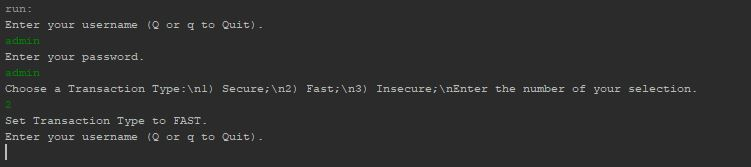
\includegraphics[width=0.6\linewidth]{./Resources/cli-admin.jpg}
	\caption{Administrator Options} \label{fig:admin}
\end{figure}

\subsection{Making a Transaction}

A user may make a transaction with the currently selected transaction mode. The user logs in with their credentials (see Figure~\ref{fig:userCreds}), and is notified which transaction mode is in use on a successful login. The user can choose to logout, or make a new transaction (see Figure~\ref{fig:menu}), and enters the amount and destination of the transfer as seen in Figure~\ref{fig:transfer}.

\begin{figure}[h!]
	\centering
	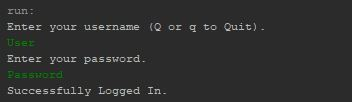
\includegraphics[width=0.4\linewidth]{./Resources/cli-login.jpg}
	\caption{User Login.} \label{fig:userCreds}
\end{figure}

\begin{figure}[h!]
	\centering
	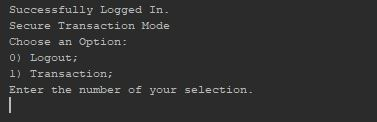
\includegraphics[width=0.4\linewidth]{./Resources/cli-loginSuccess.jpg}
	\caption{Successful Login.} \label{fig:menu}
\end{figure}


\begin{figure}[h!]
	\centering
	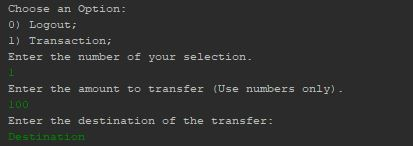
\includegraphics[width=0.4\linewidth]{./Resources/cli-details.jpg}
	\caption{Transfer Details.} \label{fig:transfer}
\end{figure}

\subsubsection{Secure Transaction Mode}

If the system is in Secure Transaction mode, the user's information is encrypted before the transaction is completed (Figure~\ref{fig:secure}).

\begin{figure}[h!]
	\centering
	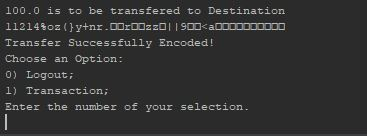
\includegraphics[width=0.4\linewidth]{./Resources/cli-secure.jpg}
	\caption{Secure Transfer.} \label{fig:secure}
\end{figure}

\subsubsection{Fast Transaction Mode}

If the system is in Fast Transaction mode, the transfer completes immediately (Figure~\ref{fig:fast}).

\begin{figure}[h!]
	\centering
	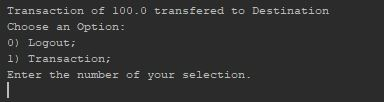
\includegraphics[width=0.4\linewidth]{./Resources/cli-fast.jpg}
	\caption{Fast Transfer} \label{fig:fast}
\end{figure}

\subsubsection{Insecure Transaction Mode}

If the system is in Insecure Transaction mode, the transfer is `hijacked' and Figure~\ref{fig:insecure} is shown to the user.

\begin{figure*}[h!]
	\centering
	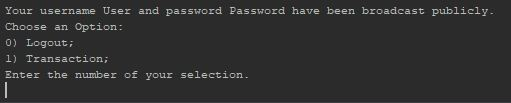
\includegraphics[width=0.4\linewidth]{./Resources/cli-bad.jpg}
	\caption{Insecure Transfer} \label{fig:insecure}
\end{figure*}


\clearpage
\section{Source Code} \label{app:code}
\setcounter{figure}{0}  
\setcounter{equation}{0} 
\setcounter{table}{0}

\lstinputlisting[language=Java, caption={PaymentApp.java}, label={src:paymentapp.java}]{../src/paymentapp/PaymentApp.java}

\lstinputlisting[language=Java, caption={PaymentService.java}, label={src:paymentservice.java}]{../src/paymentapp/PaymentService.java}

\lstinputlisting[language=Java, caption={PaymentServiceModule.java}, label={src:paymentservicemodule.java}]{../src/paymentapp/PaymentServiceModule.java}

\lstinputlisting[language=Java, caption={Transaction.java}, label={src:transaction.java}]{../src/paymentapp/Transaction.java}

\lstinputlisting[language=Java, caption={SecureTransaction.java}, label={src:securetransaction.java}]{../src/paymentapp/SecureTransaction.java}

\lstinputlisting[language=Java, caption={FastTransaction.java}, label={src:fasttransaction.java}]{../src/paymentapp/FastTransaction.java}

\lstinputlisting[language=Java, caption={InsecureTransaction.java}, label={src:insecuretransaction.java}]{../src/paymentapp/InsecureTransaction.java}

\lstinputlisting[language=Java, caption={TransactionProvider.java}, label={src:transactionprovider.java}]{../src/paymentapp/TransactionProvider.java}

\lstinputlisting[language=Java, caption={TransactionType.java}, label={src:transactiontype.java}]{../src/paymentapp/TransactionType.java}


	
\end{document}